\documentclass[pdflatex,compress]{beamer}

%\usetheme[dark,framenumber,totalframenumber]{ElektroITK}
\usetheme[darktitle,framenumber,totalframenumber]{ElektroITK}
\usepackage{graphicx}
\usepackage{multicol}

\title{Data Communications}

\subtitle{Physical Layer}

\author{Mifta Nur Farid}

\date{24 January 2024}

\begin{document}

\maketitle

\begin{frame}{Communication at the physical layer}
	\begin{center}
		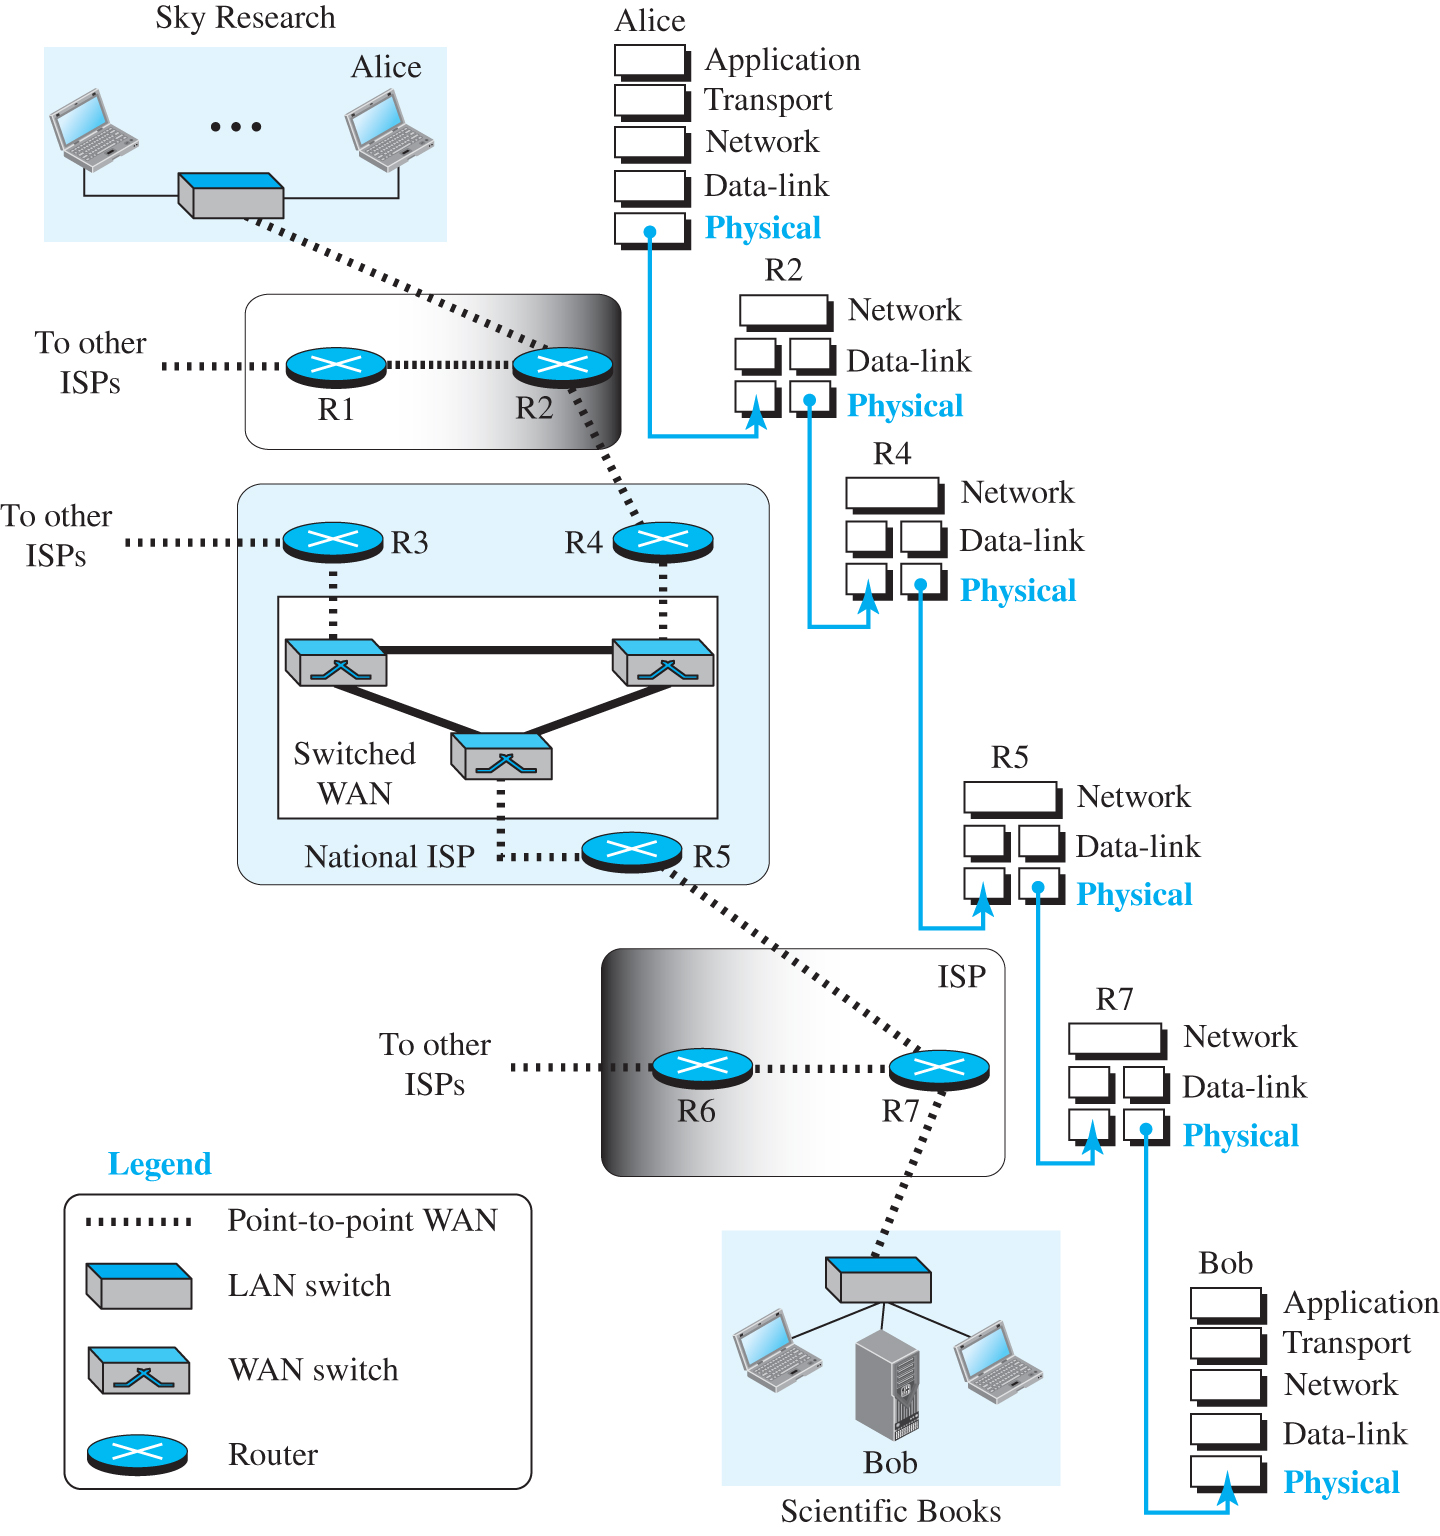
\includegraphics[height=0.8\textheight]{img/01}
	\end{center}
	\hyperlink{comm_physical_layer}{\tiny Explanation}
	\hypertarget{graph_physical_layer}
\end{frame}

\begin{frame}{Signals}
	\begin{itemize}
		\item What is exchanged between Alice and Bob is data, but what goes through the network at the physical layer is signals.
	\end{itemize}
\end{frame}

\begin{frame}{Comparison of analog and\\digital signals}
	\begin{center}
		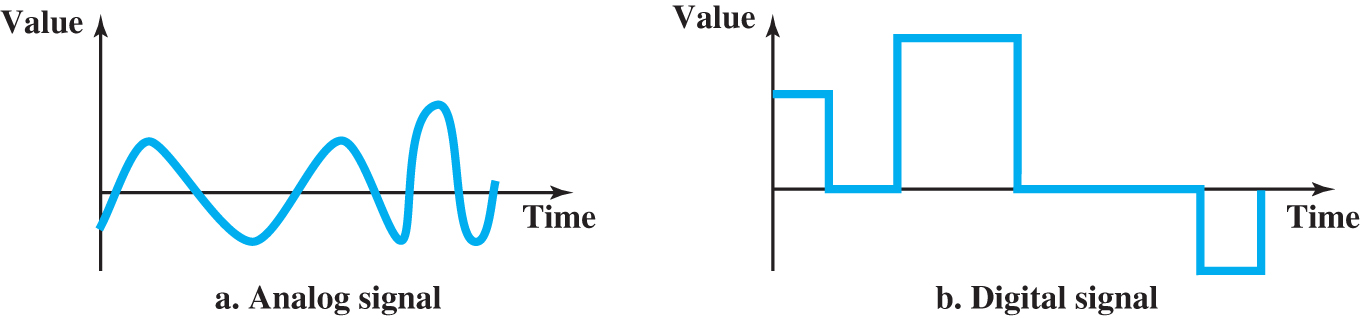
\includegraphics[width=\linewidth]{img/02}
	\end{center}
\end{frame}

\begin{frame}{Analog Signal}
	\begin{itemize}
		\item An analog signal can take one of the two forms: periodic or aperiodic. In data communication, we normally use periodic signals. A simple periodic signal, a sine wave, cannot be decomposed into simpler signals.
	\end{itemize}
\end{frame}

\begin{frame}
	\centering
	THANK YOU
\end{frame}

% ------------ TEXT --------------------- %

\begin{frame}{Comparison of analog and\\digital signals}
	\hypertarget{comm_physical_layer}
	\hyperlink{graph_physical_layer}{link text}
\end{frame}

\end{document}
